% TODO add tech / software table?
\section{Materials and methods}

\subsection{Study design}

The study had two main goals.
Firstly, I aimed to develop a map interface for
interactively presenting an extensive spatial dataset on travel times,
and through the development process assess
the tools and options available for making such a map.
More precisely,
I focused on the choice of web mapping library
and on the different approaches in preprocessing the mapped data.
The goal was to find how,
and to what extent,
these factors affect the map interface.
The second goal was to understand how map users utilize such a map interface,
and how the interactive map works as a representation.
Here I employed a survey to find out how
people use the map when given different tasks to complete with it,
and whether a highly interactive presentation approach affects
how map users perceives and interprets the mapped phenomenon.
These two themes, the development process and the survey,
make up the two high-level components of the study.

% While the primary goal of the development process was
% to produce the map presentation and enable the survey,
% the development process in and of itself was crucial to the study as well.
% Its purpose was to be the framework that
% allows for answering the research questions
% about the more technology-centric aspects of
% the making of an interactive map.

Pragmatically speaking, a large part of this study was
a software development project to produce a functional web map application,
and the parts that were not, were still reliant on
the software development project succeeding.
This naturally affected the study design.
It allowed for freedom in crafting a map interface made exactly for this study,
but also introduced limitations
as any functionality to be included in the map, and in the study,
had to also be implemented.
In other words, the technical implementation as well as the survey
had to be designed around what is meaningful to study,
but also based on what is realistic to implement.
To minimize the risk and uncertainty inherent to such a setting,
I heavily utilized modern software development methodologies
\parencite{saq2020, bec2001, sha2017, kuh2017}
in planning the development process and the study as a whole.
Based on these,
I formatted the following points of focus
to guide the development process:
\begin{itemize}
	\item Plan minimally and adapt the plan constantly.
	\item Prioritize a working state of the entire system over details in single components.
	\item Adapt to technical constraints at the start, not at the end.
\end{itemize}

By adhering to these principles I could at an early stage see
whether the study was realistic, and,
especially considering the more technology-centric side of the study,
hone in on what research questions were actually meaningful.
Iteratively improving the system as a functional whole
allowed me to consider the map interface
from the perspective of the map user as early as possible,
better integrating the survey into the study.
This is important as the map presentation is simultaneously an output of the development process
and an input to the design of the survey.

For an overview of the study design see figure \ref{fig:study design}.
% This allowed me to improve the relevancy of my research. TODO Discussion?
% I say this not only in the context of gaining valuable results to my research questions --
% I want to emphasize that to even know what research questions to ask is impossible with a linear approach.

% While the development process and the survey were linked to each other,
% they each had their separate goals and outputs too.
% In addition to producing the map presentation,
% the development process had to enable testing and answering my research questions
% about the making of an interactive map.
% This placed increased
% The goal of the survey is to gain insight on
% how the interactive map works as a representation of the mapped phenomenon.
% With the survey I collect data on map usage,
% which I in turn analyse to answer my research questions related to the map usage.

\begin{figure}[H]
	\centering
	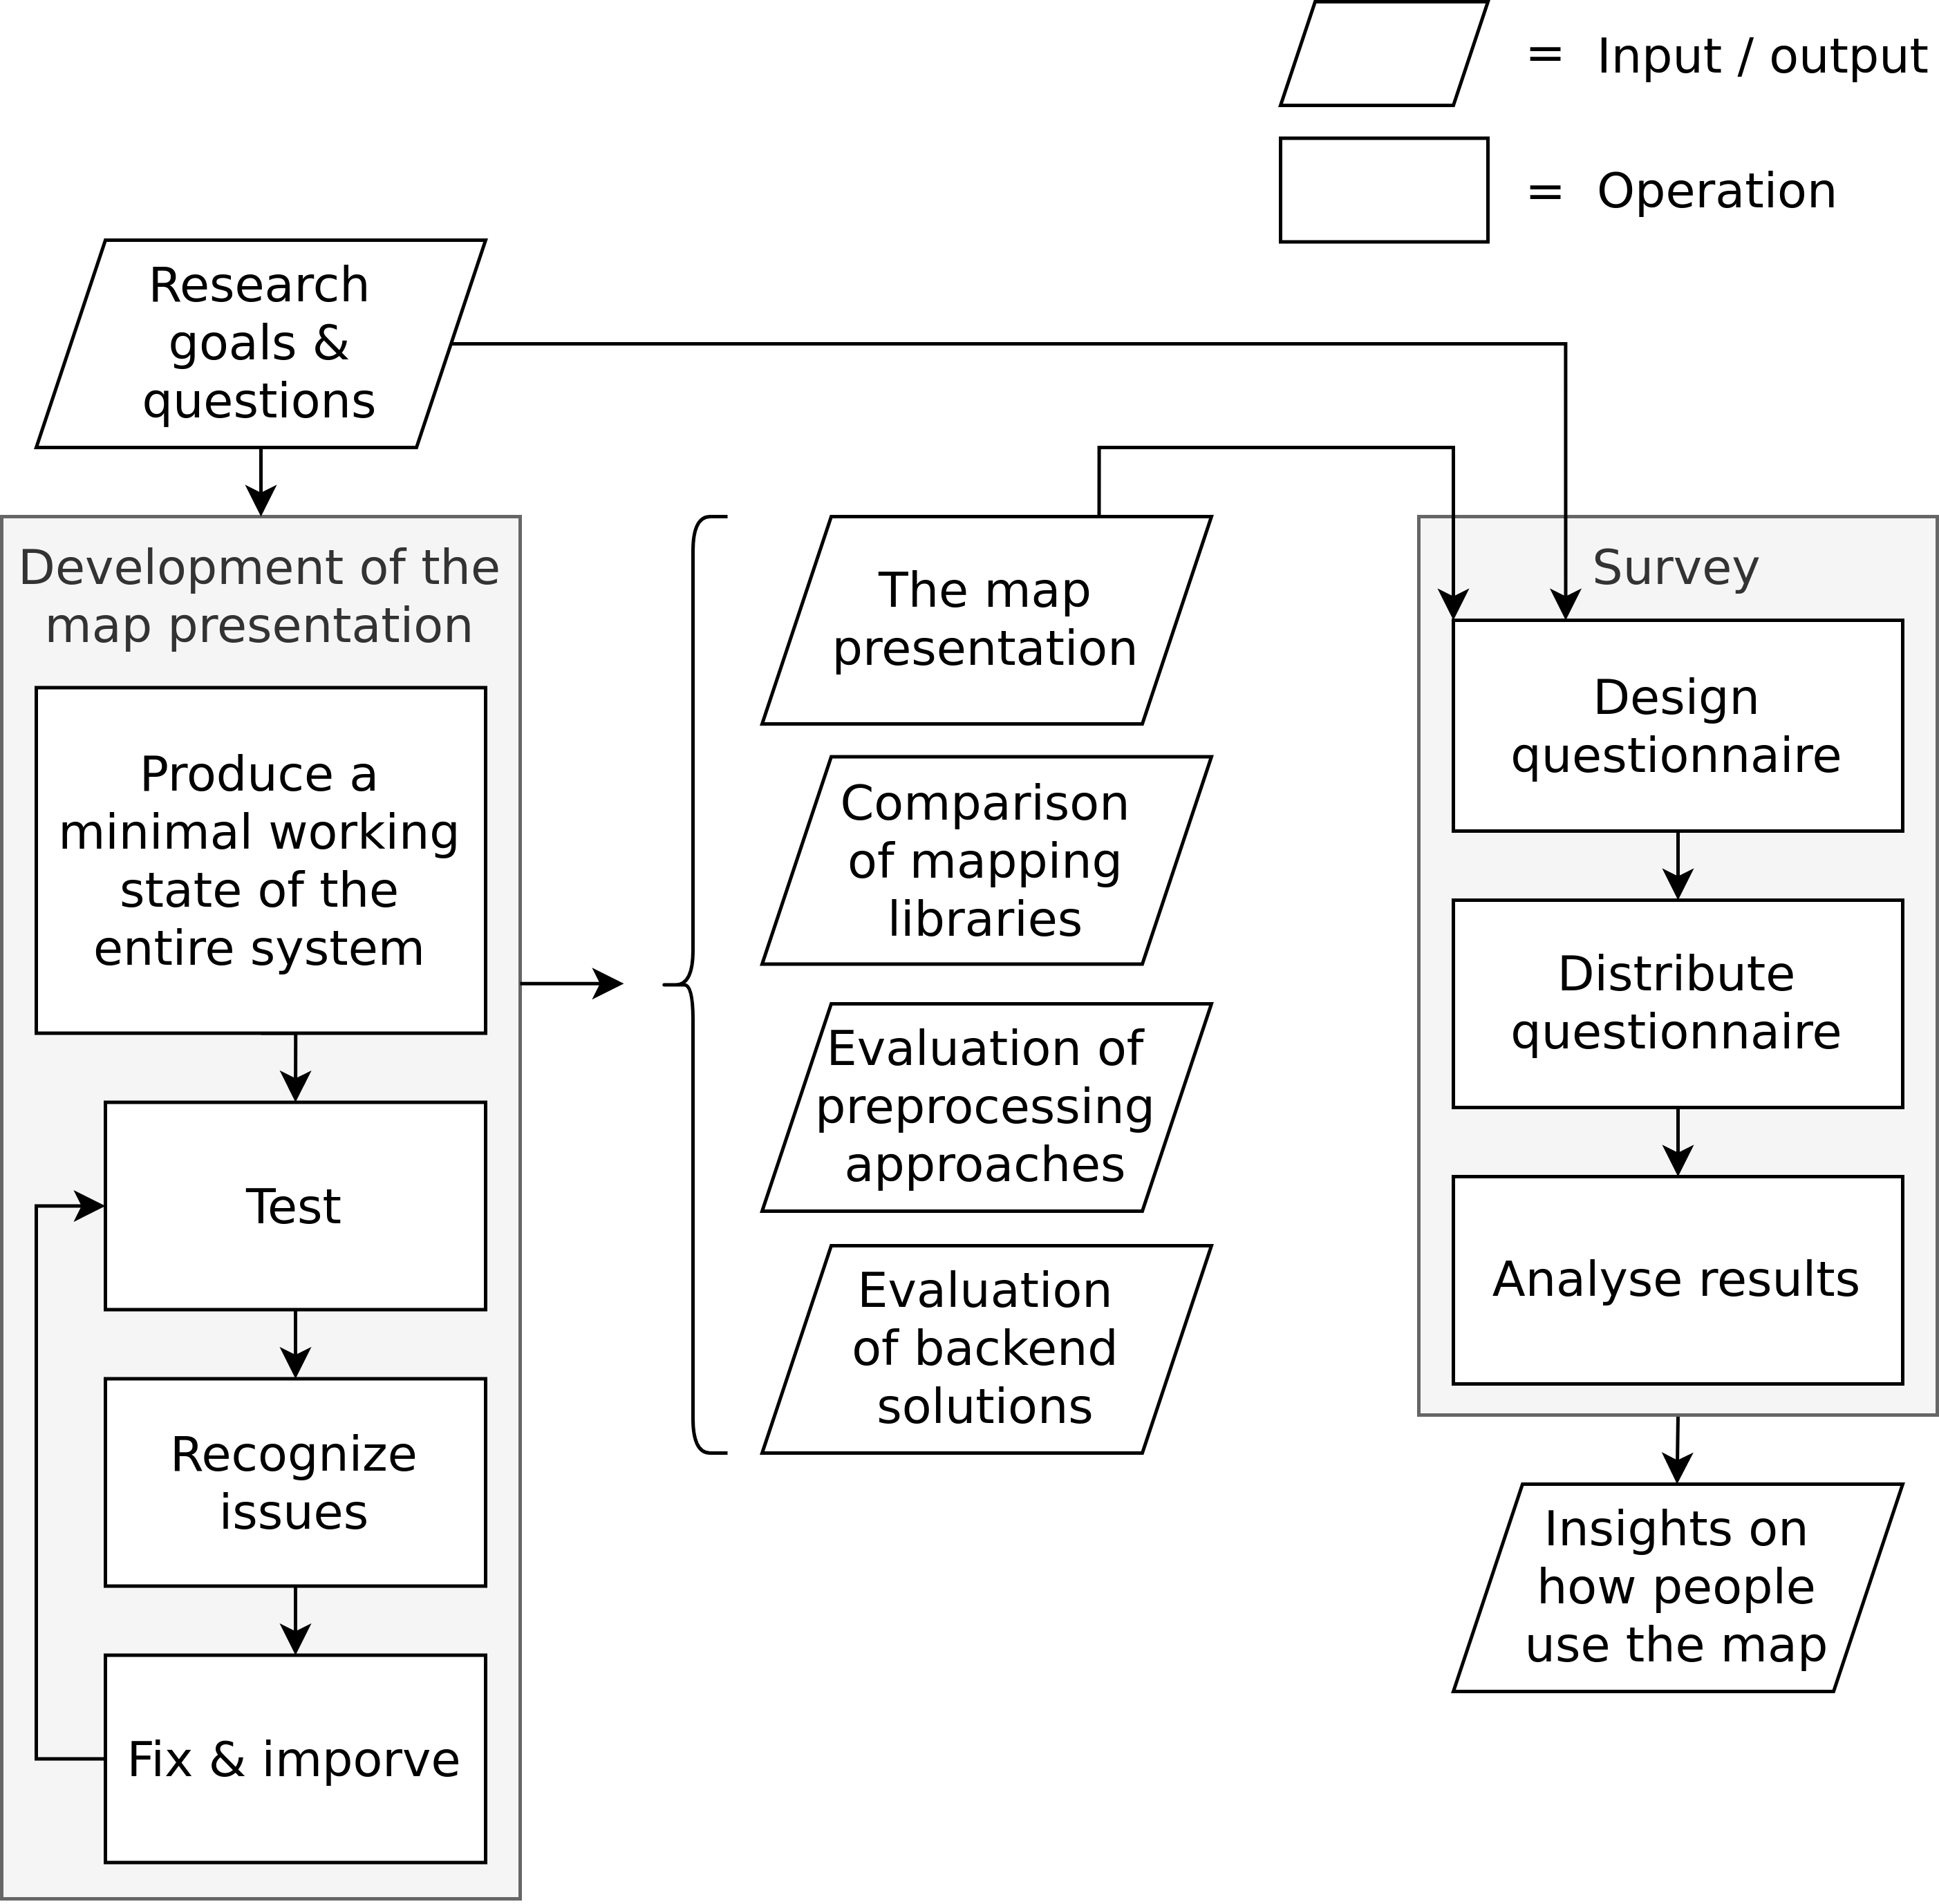
\includegraphics[width=\diagramwidth]{visual/figures/diagrams/study_design.png}
	\caption{An overview of the study design.}
	\label{fig:study design}
\end{figure}


\subsection{Data -- Helsinki region Travel Time Matrix}

The \acrlong{ttm} (\acrshort{ttm}) \parencite{fin2023}
is a dataset containing information of travel times and distances
in the Helsinki region in southern Finland.
This dataset was crucial to developing the map application,
as it was the sole source of the travel times shown on the map.
The dataset and the set of methods with which it is produced are open-source.

% Describe ttm in general: ykr, origin dest pairs etc (more surface level stuff common to all matrices)
A significant component of the \acrshort{ttm} is the \acrlong{ykr} (\acrshort{ykr})
statistical grid made by the Finnish Environmental Institute.
The grid has a spatial resolution of 250x250m, and it covers the entire Finland.
Most importantly, however, the part of the \acrshort{ykr} grid that overlaps with
the Helsinki region provides the spatial component for
the travel times stored in the \acrshort{ttm}.
The spatial extent of the dataset is shown in figure \ref{fig:ttm extent}.

\begin{figure}[H]
	\centering
	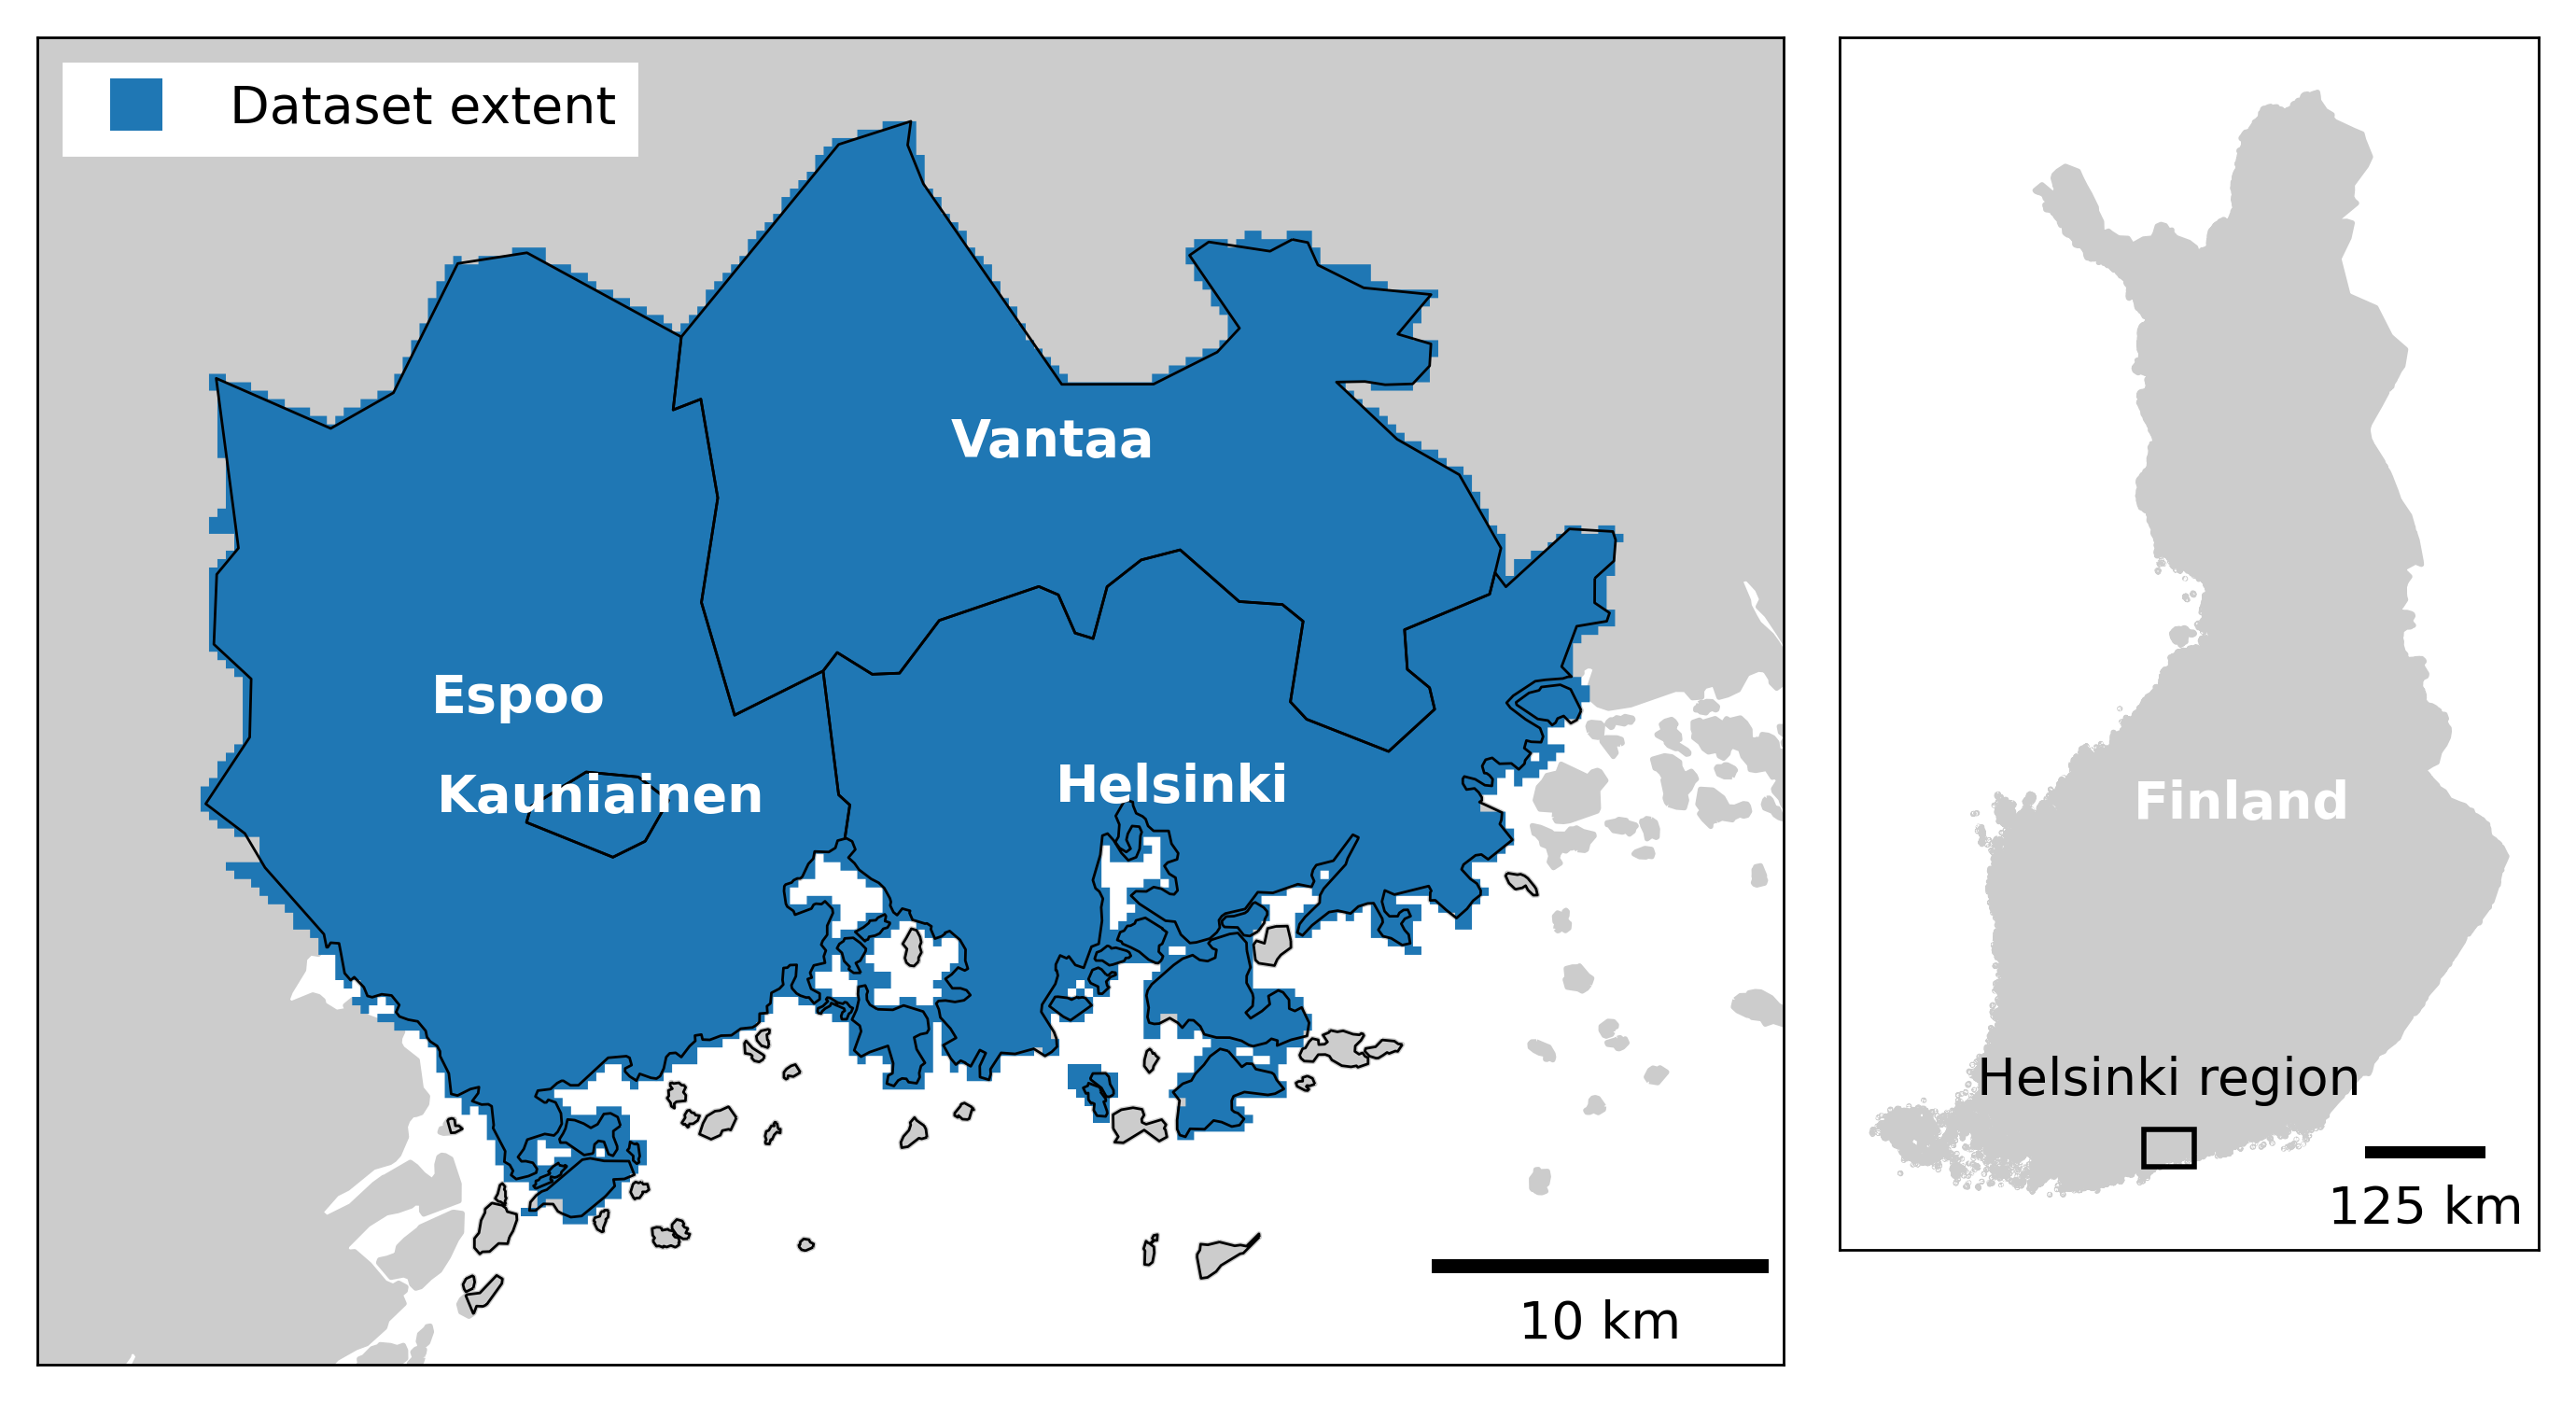
\includegraphics[width=0.9\textwidth]{visual/figures/ttm/ttm_extent}
	\caption{The location and extent of the TTM}
	\label{fig:ttm extent}
\end{figure}

The \acrshort{ttm} stores the travel times and distances
from every \acrshort{ykr} grid cell to every other  \acrshort{ykr} grid cell
within the Helsinki region.
The Helsinki region fits 13231 \acrshort{ykr} grid cells,
which means that the complete \acrshort{ttm} contains travel times and distances for
over 175 million routes.

All the routes are calculated for multiple different travel modes.
The primary travel modes are walking, cycling, public transportation and private car,
and, when applicable, each mode has variations based on
time of day and / or walking or cycling speed.
The time of day is especially relevant to motorized transport
in the form of the rush hour, for example,
while walking speed affects any travel mode
where a significant portion of the trip is covered on foot.
To be comparable with each other,
the travel times for all travel modes are
calculated with a \textit{door-to-door approach}
which accounts for things such as walking to a bus stop,
waiting for transfer times based on public transit schedules,
or locking and unlocking a bike \parencite{ten2020}.

% Describe the particular matrix (2023), methodology etc
\acrshort{ttm}s have been calculated for multiple years.
Differences between these datasets exist in the applied methodologies
and, thus, also in the content \parencite{ten2020}.
Also, the underlying city structure as well as the street and public transport networks
are by no means static over the years
which further introduces differences.
The map presentation I developed in this study
is based on the 2023 version of the \acrshort{ttm},
the newest one at the time of writing.
See table \ref{tab:ttm description} for an overview of the dataset,
and table \ref{tab:ttm table structure} for all the travel modes and
their variations included in the dataset.

\begin{table}[H]
	\caption{Descriptive values of the \acrshort{ttm}}
	\label{tab:ttm description}
	\centering
	\begin{tabular}{ | L{0.4\textwidth} | L{0.5\textwidth} | }
		\hline
		Spatial resolution
		& 250 x 250 m
		\\
		\hline
		Number of grid cells
		& 13231
		\\
		\hline
		Number of origin-destination pairs
		& 175 059 361
		\\
		\hline
		Travel modes
		& \tabitem walking \\
		& \tabitem cycling \\
		& \tabitem public transportation \\
		& \tabitem private car \\
		\hline
		Travel mode variations (if applicable)
		& \tabitem Time of day (rush hour, midday, night) \\
		& \tabitem Walking speed (average, slow) \\
		& \tabitem Cycling speed (average, fast, slow) \\
		\hline
	\end{tabular}
\end{table}


\begin{table}[H]
	\caption{The table structure of \acrshort{ttm} data}
	\label{tab:ttm table structure}
	\centering
	\begin{tabular}{ | L{0.15\textwidth} | L{0.75\textwidth} | }
		\hline
		\textbf{Column name}
		& \textbf{Description}
		\\
		\hline
		\hline
		from\_id
		& ID number of the origin grid cell
		\\
		\hline
		to\_id
		& ID number of the destination grid cell
		\\
		\hline
		walk\_avg
		& Travel time in minutes from origin to destination by walking at an average speed
		\\
		\hline
		walk\_slo
		& Travel time in minutes from origin to destination by walking slowly
		\\
		\hline
		bike\_avg
		& Travel time in minutes from origin to destination by cycling at an average speed; incl. extra time (1 min) to unlock and lock bicycle
		\\
		\hline
		bike\_fst
		& Travel time in minutes from origin to destination by cycling fast; incl. extra time (1 min) to unlock and lock bicycle
		\\
		\hline
		bike\_slo
		& Travel time in minutes from origin to destination by cycling slowly; incl. extra time (1 min) to unlock and lock bicycle
		\\
		\hline
		pt\_r\_avg
		& Travel time in minutes from origin to destination by public transportation in rush hour traffic, walking at an average speed
		\\
		\hline
		pt\_r\_slo
		& Travel time in minutes from origin to destination by public transportation in rush hour traffic, walking at a slower speed
		\\
		\hline
		pt\_m\_avg
		& Travel time in minutes from origin to destination by public transportation in midday traffic, walking at an average speed
		\\
		\hline
		pt\_m\_slo
		& Travel time in minutes from origin to destination by public transportation in midday traffic, walking at a slower speed
		\\
		\hline
		pt\_n\_avg
		& Travel time in minutes from origin to destination by public transportation in nighttime traffic, walking at an average speed
		\\
		\hline
		pt\_n\_slo
		& Travel time in minutes from origin to destination by public transportation in nighttime traffic, walking at a lower speed
		\\
		\hline
		car\_r
		& Travel time in minutes from origin to destination by private car in rush hour traffic
		\\
		\hline
		car\_m
		& Travel time in minutes from origin to destination by private car in midday traffic
		\\
		\hline
		car\_n
		& Travel time in minutes from origin to destination by private car in nighttime traffic
		\\
		\hline
		walk\_d
		& Distance from origin to destination, in metres, on foot
		\\
		\hline
	\end{tabular}
\end{table}




\subsection{Implementation of the map presentation}

\subsubsection{Software requirements}
% The requirements of the system are an essential aspect to consider,
% since they
% For example, the sheer scale and detail of the dataset being visualized
% means that instantaneous interaction with the map is not realistic
% if no detail of the mapped data is to be sacrificed.
% These kinds of tradeoffs are important to recognize,
% because only through them is it possible to specify what
% requirements should, or even could, be placed on the map application.

% TODO copypasta

% Roughly what kind of a map? Why?
% Based on the background study,  % TODO
Software requirements are the functionalities and properties
that a given system should have,
as well as the constraints it must adhere to \parencite{chu2009}.
They are an essential aspect to consider in software development
as they are a way to explicate the framework
in which an implementation process is carried out \parencite{saq2020}.
Software requirements are often divided into
functional and nonfunctional requirements.
Functional requirements define the user-facing features of the system
while nonfunctional requirements describe the properties of a system
\parencite{chu2009}.
Nonfunctional requirements can be further divided into
quality attributes and constraints.
Quality attributes describe \textit{how} the software should be,
while constraints mean technical limitations \parencite{chu2009}.

The starting point for specifying the requirements of the map interface
was the decision to prioritize real-time interaction over minute detail in the map.
The goal of the map interface was to act as a dynamic overview to the entire \acrshort{ttm}.
As mentioned in the previous section,
the spatial dimension of the \acrshort{ttm} is large.
If all of it is to be explored,
an interaction exchange to select and re-select different locations to map
should be as effortless and instantaneous as possible.
The other dimension, travel mode, is much smaller,
but should also be interactively selectable.
These two goals, while still quite vague,
immediately placed a number of requirements on the system.
From the perspective of the user,
there must be functionalities for interacting with the map to
select different locations, preferably very rapidly,
and different travel modes.
A significant quality attribute to consider is that the system should
be responsive enough for instantaneous real-time interactivity.

Another key factor was the decision to target the web as the platform.
This constraint was the starting point for considering the technologies
for carrying out the implementation.
Also, implementing a web map that visualizes a large dataset required
a solution for supplying the data to the map application:
In addition to the map interface that the user interacts with
a solution for serving data to the map application.

In accordance with the guideline of continuous adaptation
\parencite{bec2001} I specified the software requirements loosely at first,
further focusing them as the system and the study took shape.
To communicate the development and study process in an orderly manner,
and to motivate the design decisions I've made,
I present the requirements of the final system here.
Still, I should emphasize that the reality is not this linear.

The functional requirements \parentab{functional requirements}
comprise two modes of interaction for selecting locations:
clicking the map with a pointing device to produce a static map of the clicked location,
and continuously changing the location by moving the mouse over the map
(referred to as hovering).
Also, interface capabilities for selecting travel modes
and changing the mode of location selection should be present.
For the quality attributes of the system \parentab{quality attributes}
performance is an essential consideration,
both in the sense of software performance
and the responsiveness of the application as perceived by the user.
This must be considered in both the client- and server side of the system.

% TODO all refs here
Aspects that are invisible to a user, but still vital,
are that the system can be maintained and deployed,
and that it can meet different real-world usage loads \parentab{quality attributes}.
If these attributes were lacking,
the system would have little real value.
As mentioned earlier,
the client-side application is constrained to running in a web browser \parentab{constraints}.
The \textit{deployment environment},
in other words the computing platform onto which the server-side of the system is deployed,
is the container orchestration platform \textit{Rahti} provided by the \presentacr{csc}.
In short, containerization refers to a set of technologies
that enables packaging software and all its necessary components
into self-contained \textit{container images} that can be run as is,
regardless of the specifics of the underlying system.
Rahti is based on the \textit{OpenShift} platform,
which in turn runs on \textit{Kubernetes}.
Kubernetes is a container orchestration tool
that allows for declaratively managing clusters
of containerized applications and their accompanying services.
To recap what all this means for the constraints of the application:
The implementation must be completely containerized,
and the server-side is managed with the OpenShift flavour of Kubernetes
\parentab{constraints}.

\begin{table}[H]
	\caption{The functional requirements of the map application}
	\label{tab:functional requirements}
	\centering
	\begin{tabular}{ | L{0.3\textwidth} | L{0.6\textwidth} | }
		\hline
		Requirement
		& Description
		\\
		\hline
		\hline
		Location selection by clicking
		& The user can click on a location and produce an accessibility map of that location.
		\\
		\hline
		Location selection by hovering
		& The user can hover their mouse over the map,
		and the map shows the accessibility of the location that is under the cursor,
		updating constantly as the cursor moves.
		\\
		\hline
		Toggling between modes of location selection
		& The user can toggle their mode of interaction by clicking:
		Clicking while hovering locks the map, clicking while the map is locked resumes hovering.
		\\
		\hline
		Interactive selection of travel mode
		& The user can choose the travel mode for which the travel times shown on the map are calculated.
		\\
		\hline
	\end{tabular}
\end{table}

\begin{table}[H]
	\caption{
		The nonfunctional requirements of the map application specify
		its desired qualities (\ref{tab:quality attributes}) and
		the constraints it must adhere to (\ref{tab:constraints}).
	}
	\label{tab:nonfunctional requirements}
	\begin{subtable}[h]{\textwidth}
		\caption{}
		\label{tab:quality attributes}
		\centering
		\begin{tabular}{ | L{0.2\textwidth} | L{0.7\textwidth} | }
			\hline
			\textbf{Category}
			& \textbf{Requirements}
			\\
			\hline
			\hline
			Performance
			& \tabitem Data serving speed allows for real-time interaction. \\
			& \tabitem Map rendering speed allows for real-time interaction. \\
			\hline
			Maintainability
			& \tabitem All components are as independent as possible. \\
			& \tabitem The codebase is versioned and documented. \\
			& \tabitem Deploying the application is reproducible. \\
			\hline
			Usability
			& \tabitem Visual feedback from user interaction is instantaneous. \\
			\hline
			Scalability
			& \tabitem The application is scalable to meet different usage loads. \\
			& \tabitem Different application components can be scaled independently. \\
			\hline
		\end{tabular}
	\end{subtable}
	\newline
	\newline  % https://tex.stackexchange.com/questions/38893/cant-generate-vertical-space-between-tables
	\newline
	\begin{subtable}[h]{\textwidth}
		\caption{}
		\label{tab:constraints}
		\centering
		\begin{tabular}{ | L{0.2\textwidth} | L{0.7\textwidth} | }
			\hline
			\textbf{Type of constraint}
			& \textbf{Description}
			\\
			\hline
			\hline
			Client-side platform
			& The frontend of the map application runs in a web browser.
			\\
			\hline
			Deployment environment
			& The front and backend are deployed in containers
			utilizing the OpenShift container platform.
			\\
			\hline
		\end{tabular}
	\end{subtable}
\end{table}


\subsubsection{Assessing data preprocessing approaches}
% The need for preprocessing
% - what would raw data be like?
% - why as much as possible should be precalculated
% && the requirements preprocessing must satisfy
Preprocessing and simplifying the \acrshort{ttm} was a significant part of the study.
Soon after starting the development,
it became obvious that using unprocessed \acrshort{ttm} data was not an option
due to the unresponsiveness of rendering and the large file sizes.
Because of this, in the initial testing phase of the development
I formed the hypothesis that either file sizes
or the geometrical complexity of the data would be
the major factor limiting the responsiveness of the map,
i.e. the performance bottleneck.

So it was clear that some type and level of simplification of the 
data was necessary to enable real-time interaction in the map.
The goal of my assessment of different approaches to data preprocessing, thus,
was to find the suitable level and types of simplification,
and to compare the effectiveness of different approaches.

When assessing the preprocessing approaches, I focused on:
\begin{enumerate}
	\item The impact on file size, and thus on the speed of transferring data over internet.
	\item The impact on rendering speed of the map when mapping the data.
	\item The impact on the visual detail of data,
	i.e. how much information is lost.
\end{enumerate}

I assessed four preprocessing approaches:
\begin{enumerate}
	\item Aggregation of travel time data into isochrones (figure \ref{fig:isochrone intervals})
	\item Limiting the maximum travel time, i.e. the geographical extent of the results (no figure yet)
	\item Reducing geometry precision
	\item File structure optimizations (simplifying GeoJSON structure, compression using gzip)
\end{enumerate}

To carry out the assessment
I constructed a modular Python-based preprocessing pipeline
(figure \ref{fig:preprocessing}).
The idea was that the complete pipeline applies all preprocessing approaches,
but the modular design allows for
isolated testing of the
different components of the pipeline, with different parameters.

\begin{figure}[H]
	\centering
	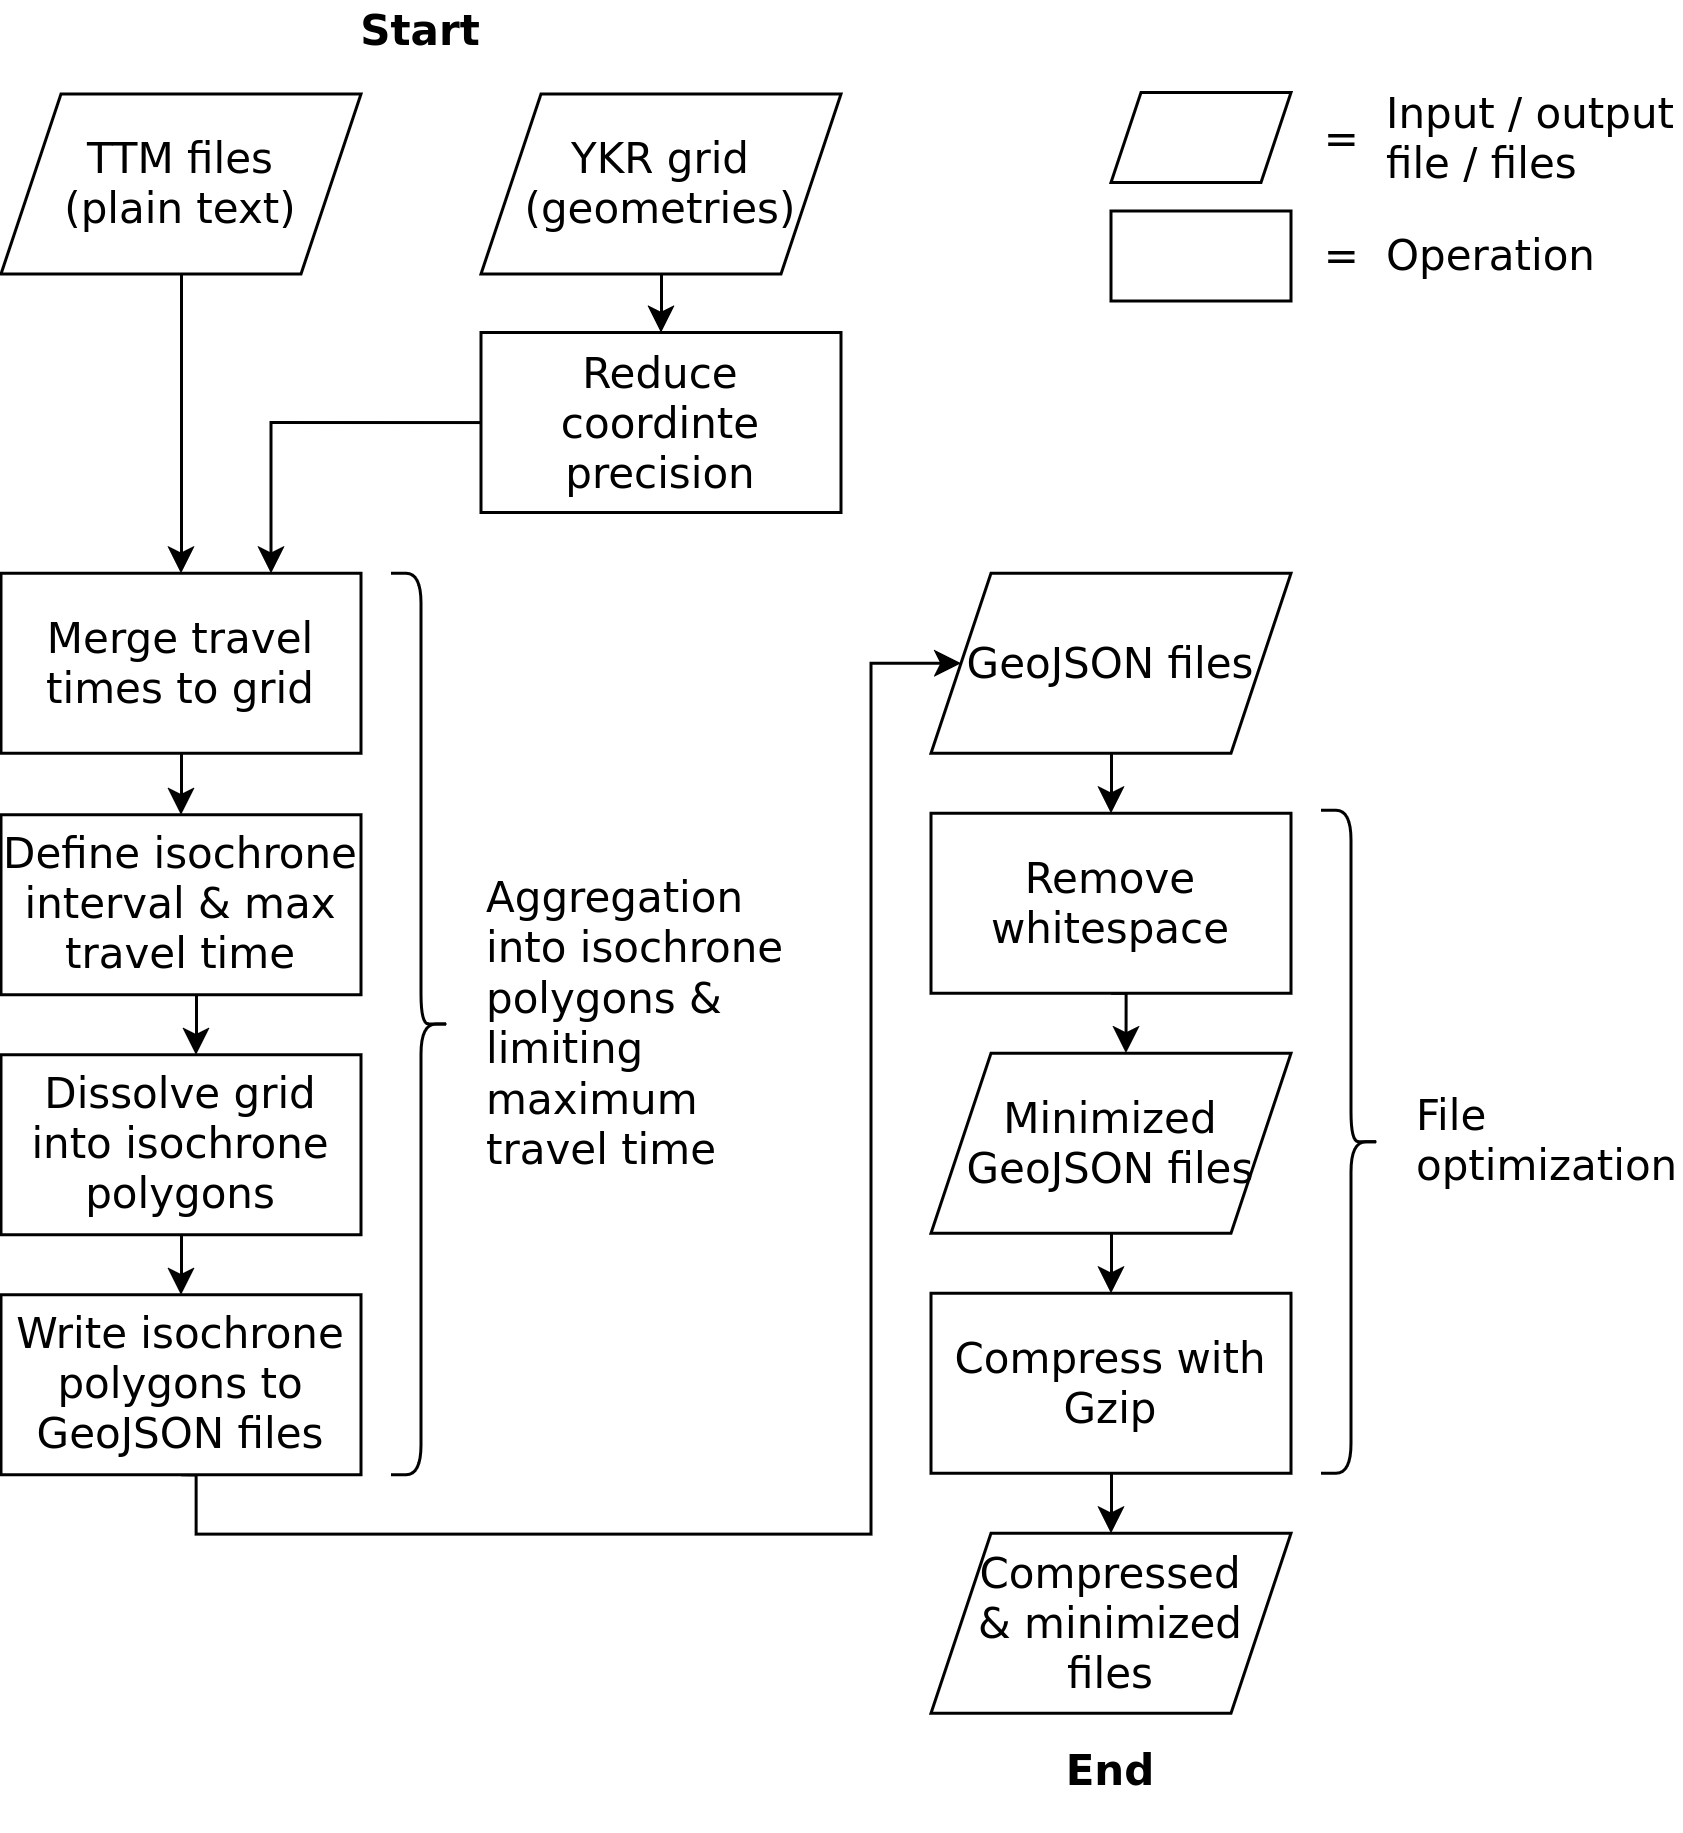
\includegraphics[width=\diagramwidth]{visual/figures/diagrams/preprocessing.png}
	\caption{Preprocessing}
	\label{fig:preprocessing}
\end{figure}

File sizes were the simplest factor to test for.
I tested each approach on
a randomly picked set of 100 locations in the \acrshort{ttm},
for each travel mode.
I picked a random sample of locations since the
data is of a different level of complexity based on location.
To measure the effect on file size I then calculated the mean file size it takes to represent
all the travel modes for a single cell in the dataset
when a given approach has been applied.

SIDENOTE: Filesize tests are in a notebook here: https://github.com/eemilhaa/travel-time-matrix-visualisation-preprocessing/blob/cleanup/example.ipynb.

I assessed the impact the preprocessing approaches have on rendering speed
with the finished map application.
The details of the map application are in the next section.
The assessment was qualitative,
as it was based on my own perception of responsiveness when using the map.
Quantitative testing of rendering speed would have been preferable,
but it proved to be difficult.
While tools for profiling rendering speed exist,
I did not succeed in two main areas
that would have been necessary for representative results.
I did not manage to limit the timing to strictly the map
component of the interface in such a way that
the test results would be reproducible.
I also did not find a way to automate a set of renders
on a sample of locations.
Averaging the renders of a single location would not suffice
for reasons stated above.
The tools I tried were the Firefox profiler
and the React developer tools browser extension on Firefox and Chromium
(I'll need to properly refer to these).

I carried out the assessment of the impact on visual detail of the data in two ways:
Qualitatively for all approaches by observing the simplified data on the map,
and, in the case of limiting maximum travel time,
quantitatively by calculating the percentage of the total dataset area that the simplified data covers.
I calculated these values as averages of a random sample of 100 locations, for each travel mode.

\begin{figure}[H]
	\centering
	\begin{subfigure}[b]{0.5\textwidth}
		\centering
		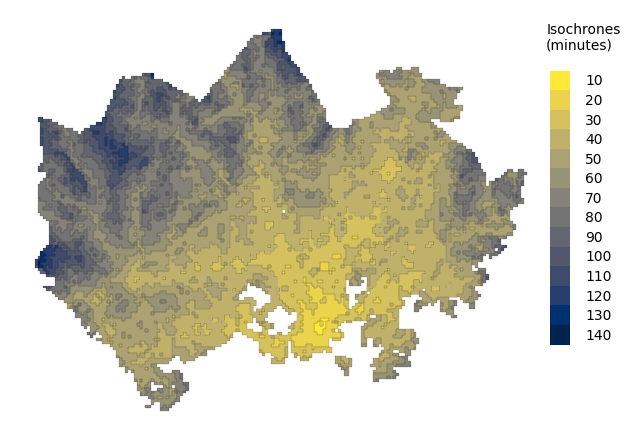
\includegraphics[width=\textwidth]{visual/figures/ttm/isochrone_interval_10}
		\caption{Isochrones with an interval of 10 minutes}
		\label{fig:interval 10}
	\end{subfigure}%
	\hfill
	\begin{subfigure}[b]{0.5\textwidth}
		\centering
		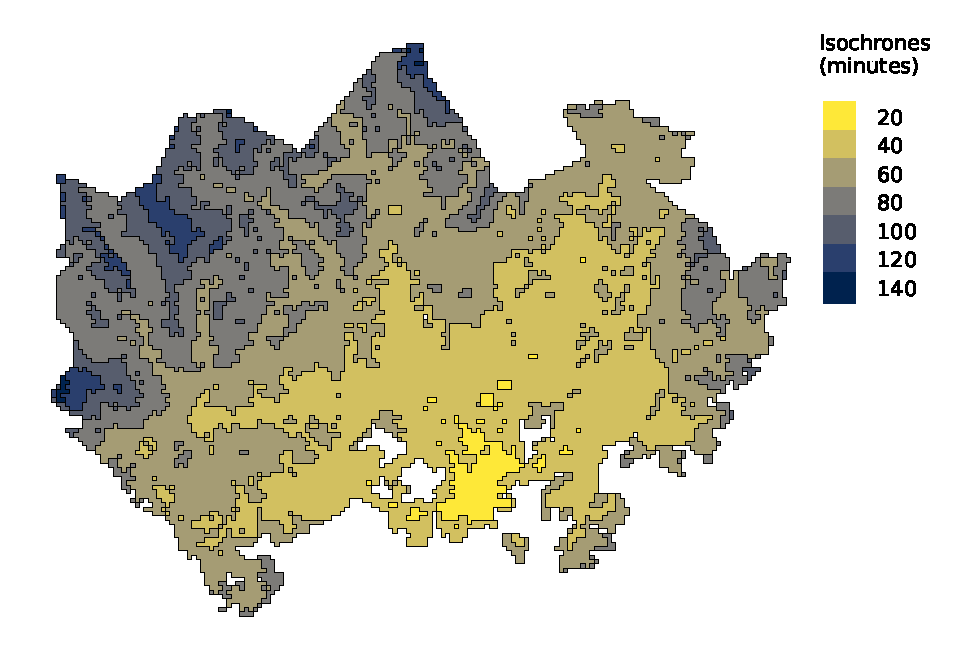
\includegraphics[width=\textwidth]{visual/figures/ttm/isochrone_interval_20}
		\caption{Isochrones with an interval of 20 minutes}
		\label{fig:interval 20}
	\end{subfigure}%
	\hfill
	\begin{subfigure}[b]{0.5\textwidth}
		\centering
		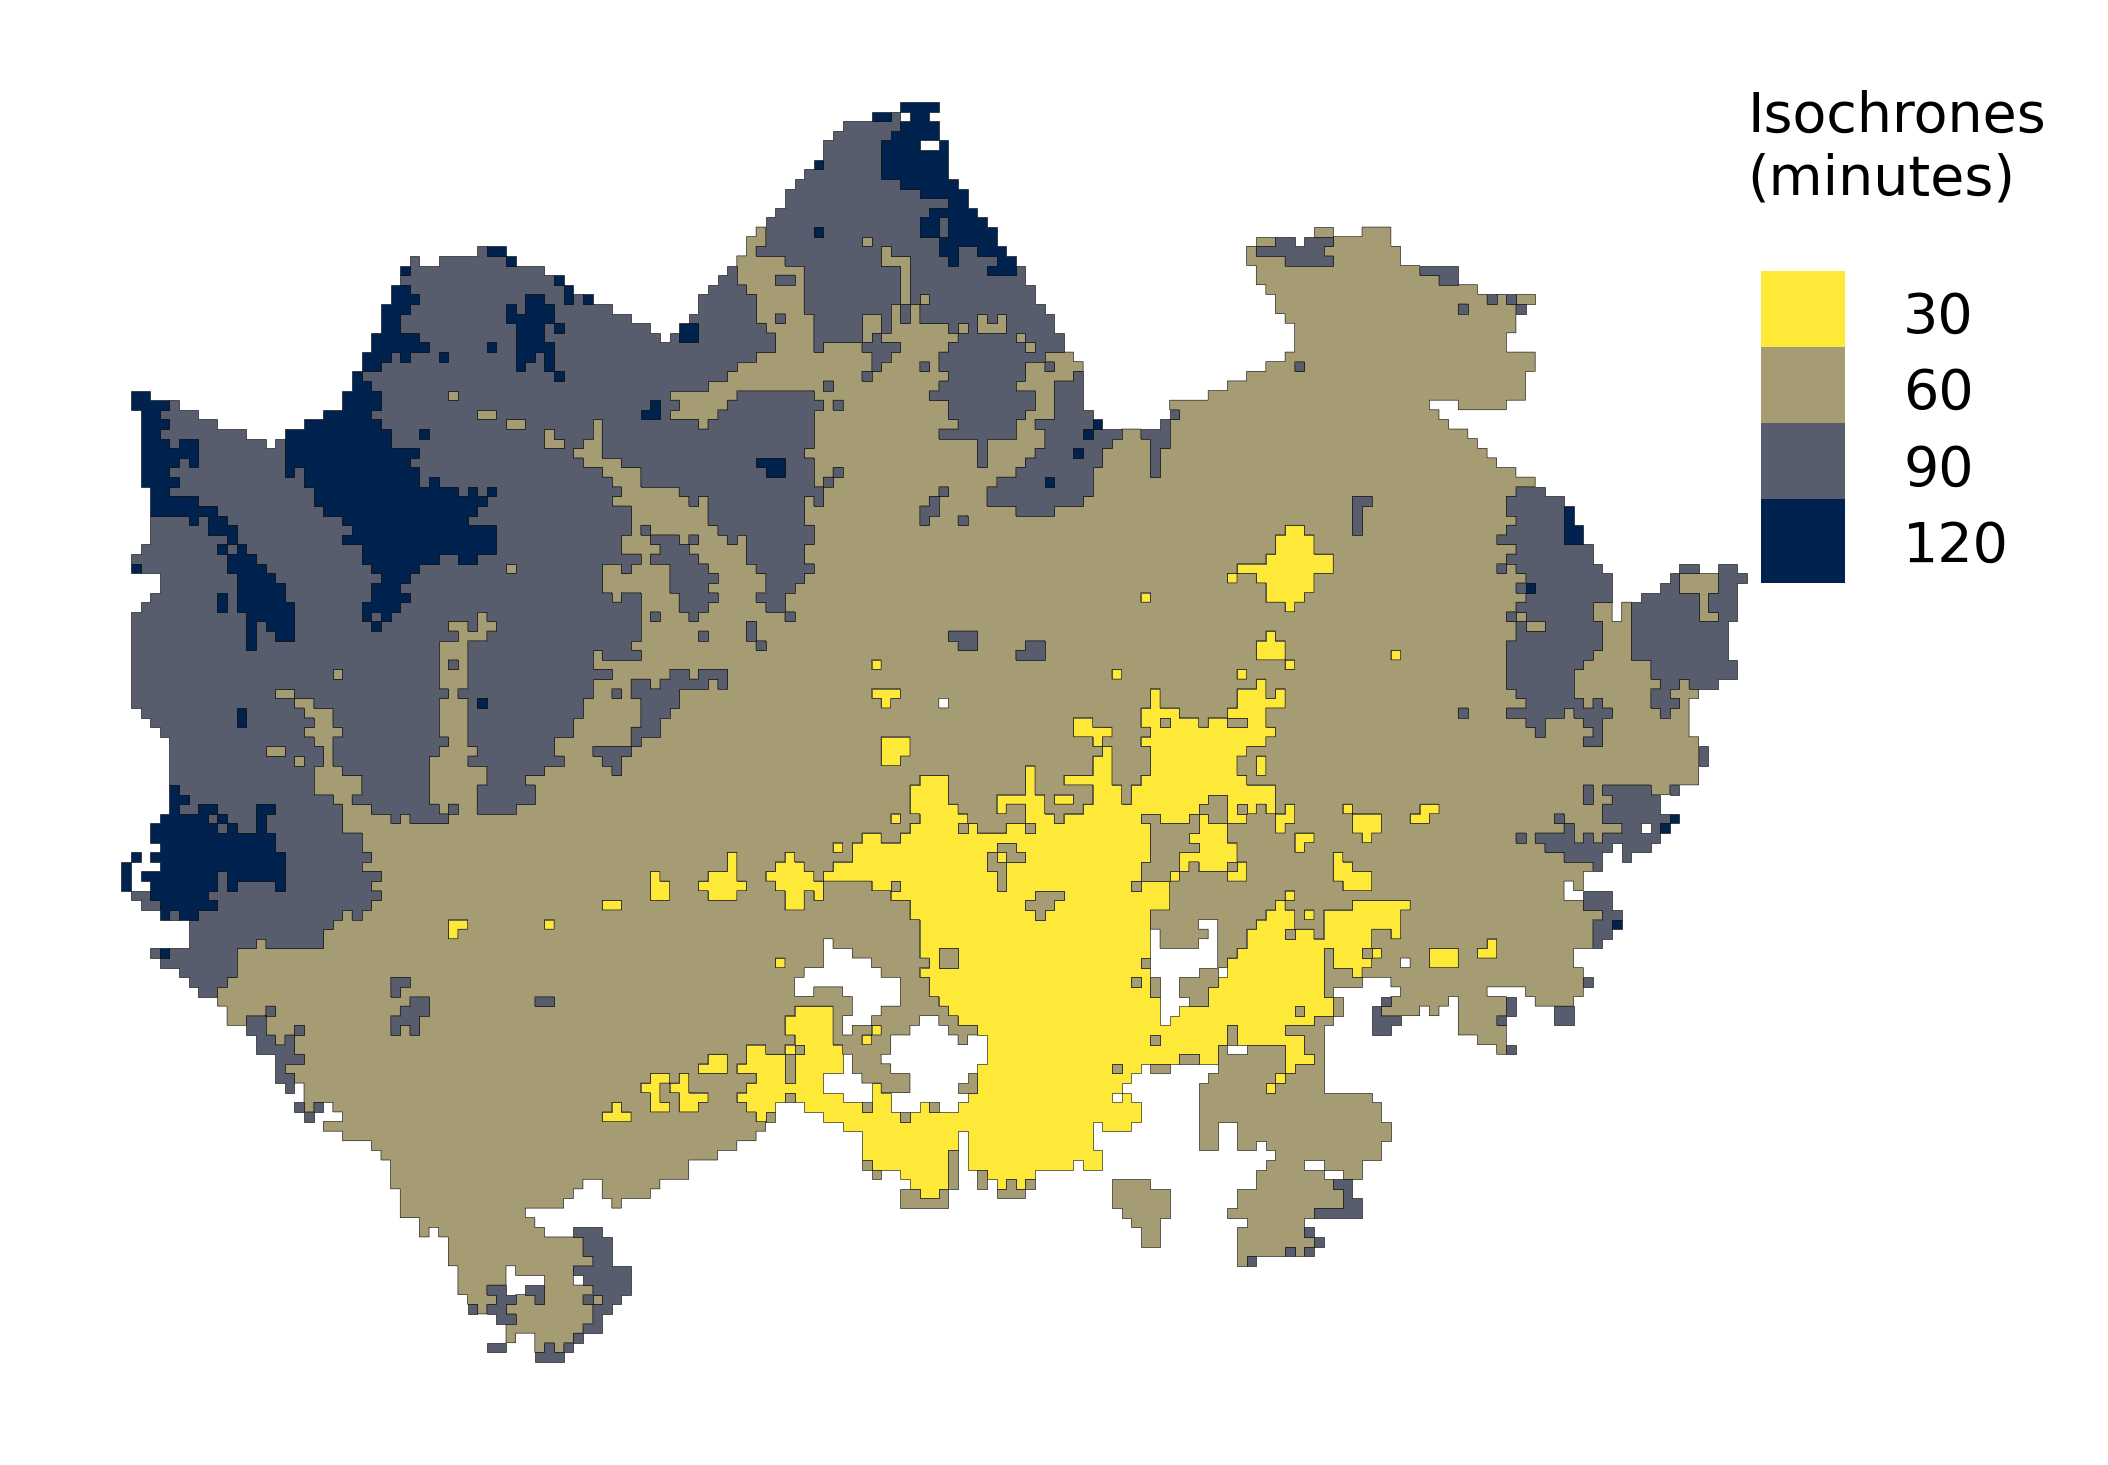
\includegraphics[width=\textwidth]{visual/figures/ttm/isochrone_interval_30}
		\caption{Isochrones with an interval of 30 minutes}
		\label{fig:interval 30}
	\end{subfigure}%
	\caption{Travel time to Helsinki railway station by public transport mapped with isochrones of different intervals}
	\label{fig:isochrone intervals}
\end{figure}

SIDENOTE: I intend to add similar figures of limiting maximum travel time here.

\subsubsection{Assessing web mapping libraries}

The solution for rendering the data to a map, i.e. the web mapping library,
was one of the most important decisions of the development process. 
In addition to rendering data correctly and efficiently,
the mapping library must allow for user interaction not only with the map,
but the underlying application.
Often, interaction with a web map changes only the state of the map,
for example by zooming,
and the web-mapping library handles an internal state change like this automatically.
With the map presentation I developed,
the map interaction must also change state outside the map.
For example:
Location selection should result in the fetching of new data from the backend,
and the mode of map interaction must be changed by map interaction.

Controlling state in web-applications is often best done by a specified solution,
such as a state store or, if applicable, a UI framework.
For this map presentation I chose to control application state with React,
as it is the most widely used and documented UI framework,
and also the only UI framework that many web-mapping libraries have integration capabilities for.
In general, integration with a framework instead of a self-made solution
means less room for error in the implementation,
and better maintainability and extensibility as the amount of code is drastically smaller.
Also, I used React in implementing the few non-map user-interface elements
(travel mode selection, legend, tooltip),
which meant no additional dependencies.

I based my assessment of web mapping libraries on three criteria:
\begin{enumerate}
	\item Visual quality of the map
	\item Responsiveness of the map
	\item Integration with React
\end{enumerate}

SIDENOTE: I don't know if I should be so technology-specific with React.
React really isn't the point, the point is that a UI framework is sensible
to not have to do everything from the ground up. React just happens to
be \textit{the} framework
(and the only framework pretty much any mapping library integrates with in any way).

When selecting which web mapping libraries to assess, I used the following properties as a baseline:
\begin{enumerate}
	\item Free and open source licensing
	\item Actively maintained
	\item At least some level of integration with React
\end{enumerate}

With these considerations I arrived at three potential libraries:
Leaflet, Maplibre and Deck.gl.
To assess the criteria above,
I used each library as the map interface with the application.
I assessed visual quality of the map qualitatively, and, for the reasons I stated in the previous chapter,
I had to resort to qualitative assessment for rendering performance as well.
For assessing integration with react additionally I utilized online documentation of potential solutions.

% % TODO copypasta
% Translucent Overlay (OV) is the best technique over-
% all, which makes it a good choice when only one comparison
% technique should be provided to user \parencite{lob2015}.


\subsubsection{Technical architecture}

\begin{itemize}
	\item Backend: Minimal HTTP sever serving pre-compressed geojson files directly from filesystem
	\item Scalable Kubernetes / OpenShift deployments → Reproducibility at the level of the entire system
	\item Containerization → Reproducibility at the level of the components of the system
	\item Modularity of the design
	\item the list goes on, I'll have to consider what matters and what doesn't.
\end{itemize}

\begin{figure}[H]
	\centering
	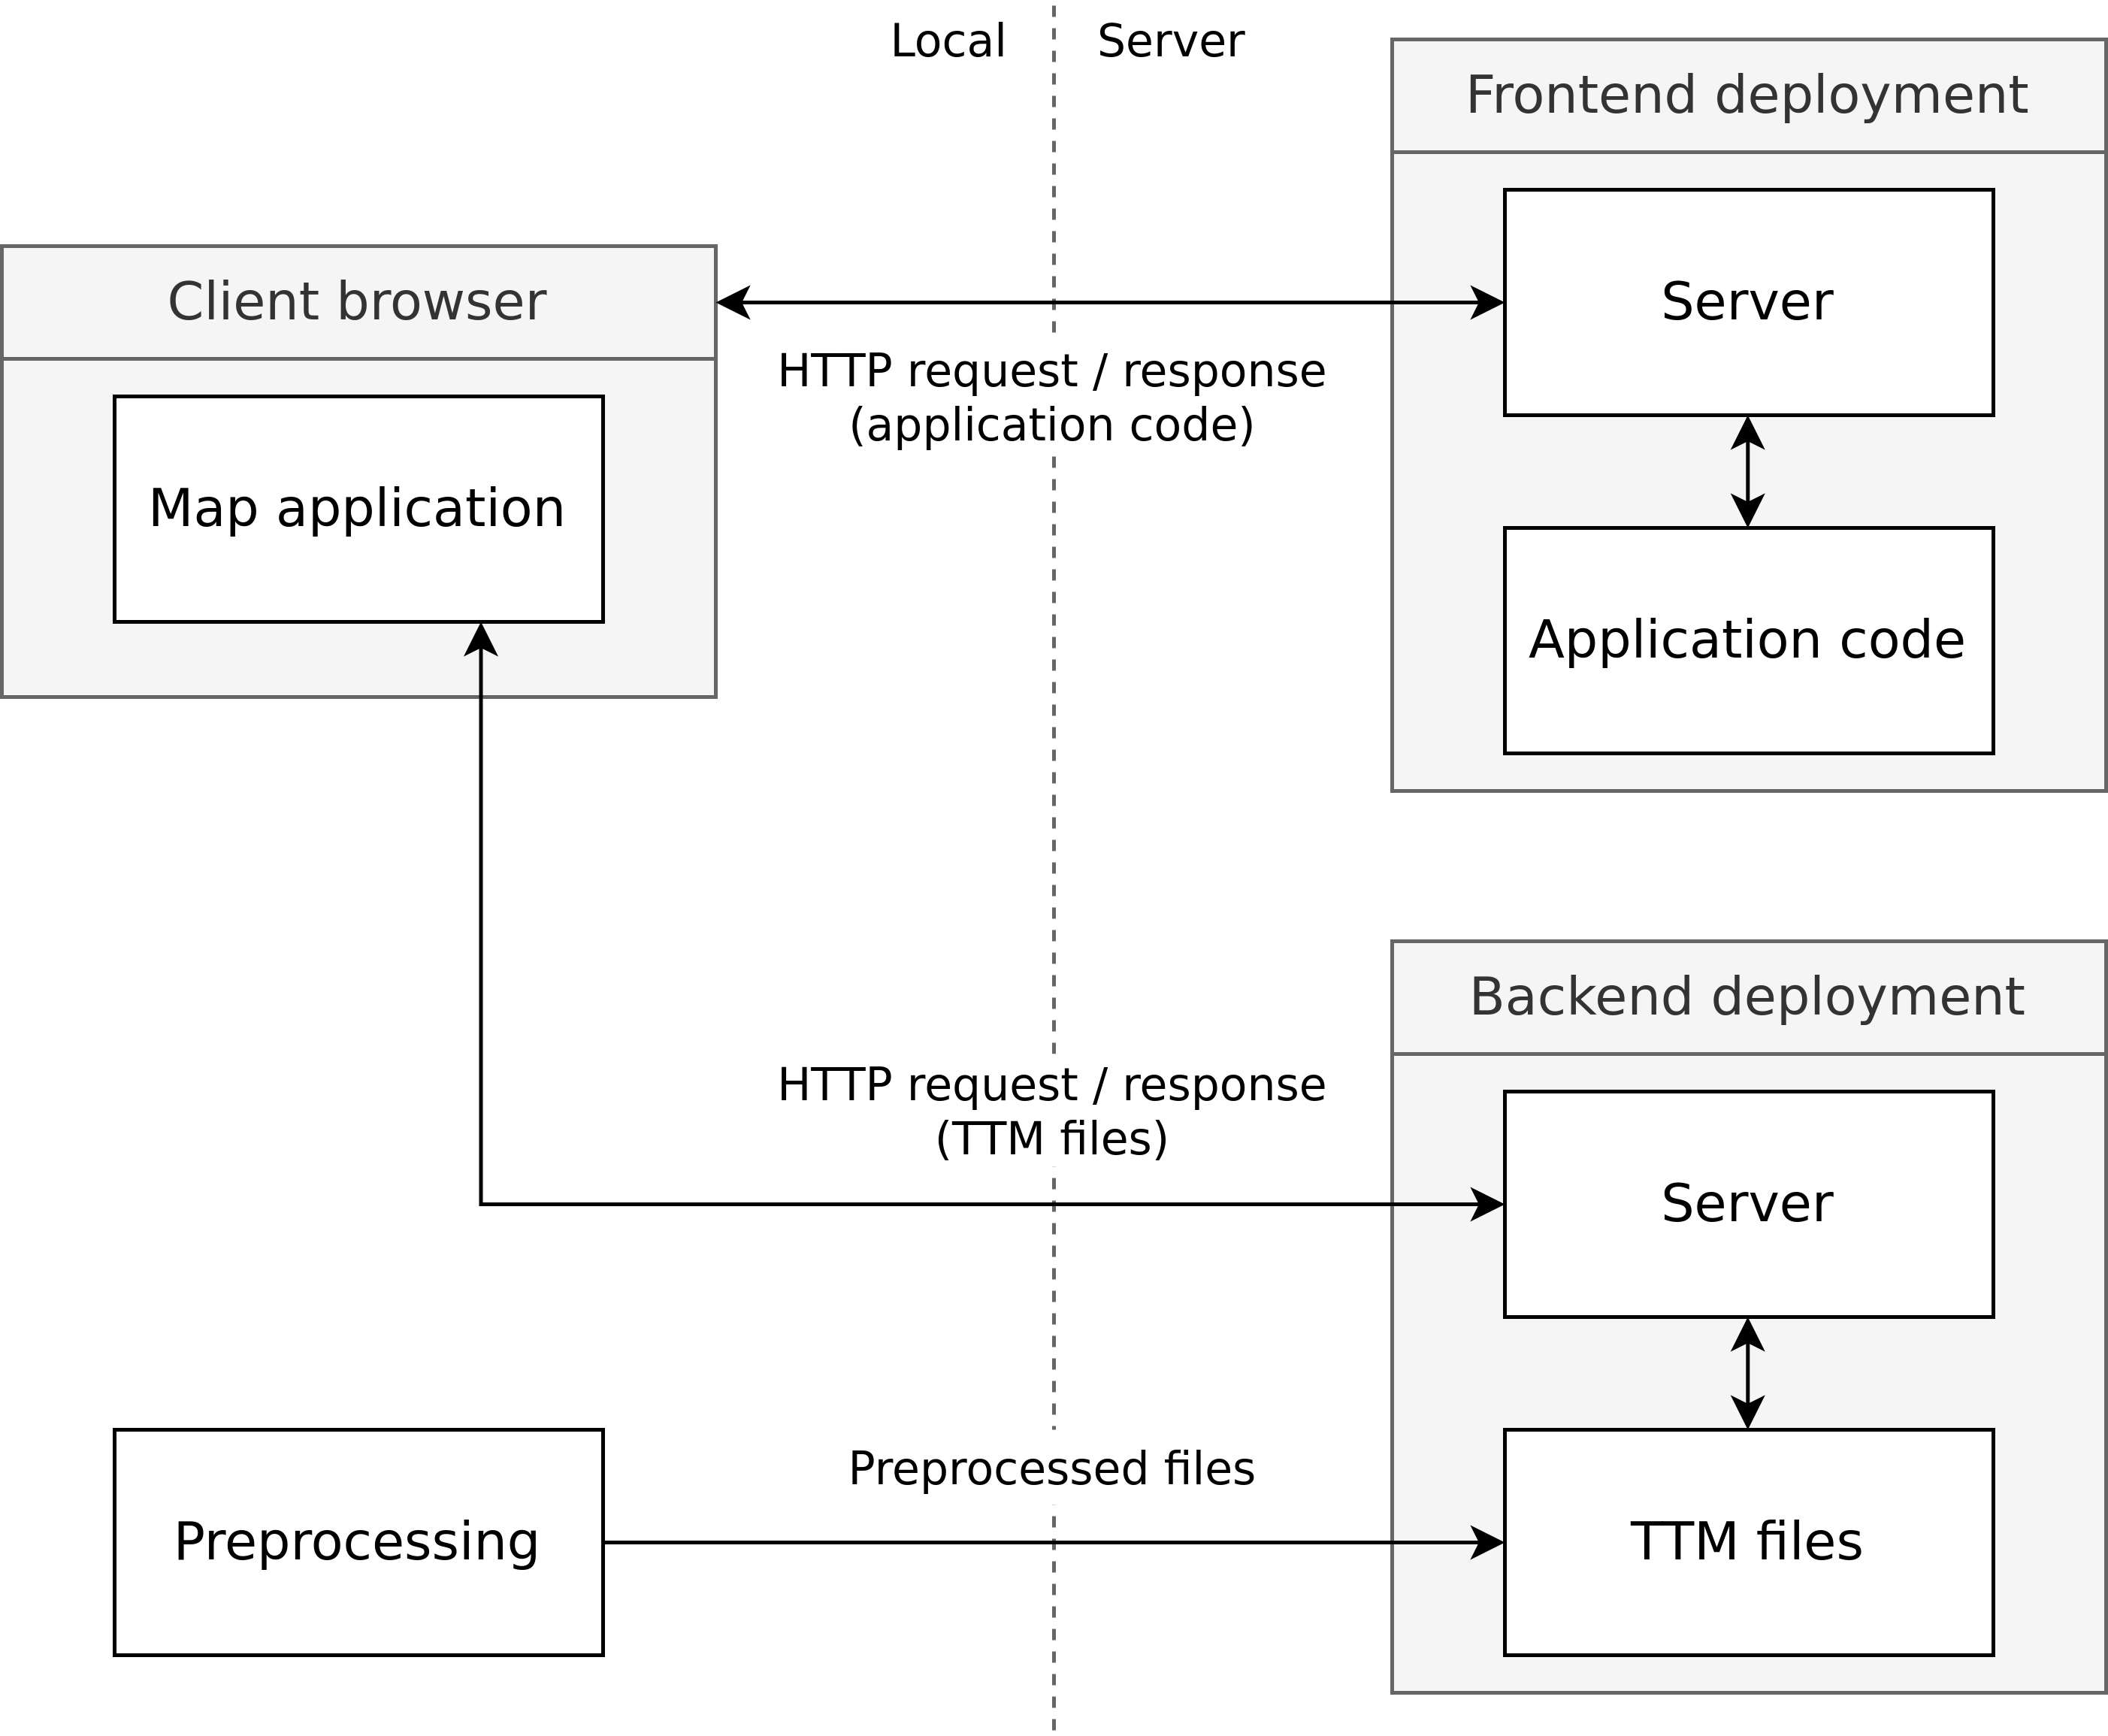
\includegraphics[width=\diagramwidth]{visual/figures/diagrams/architechture.png}
	\caption{Architecture}
	\label{fig:architechture}
\end{figure}

SIDENOTE: I'll add figures of the components (at least the map application) here as suggested by Pyry.


% The need for serving (backend)
% - why data must be decoupled
% && the requirements serving must satisfy

% Different approaches

% Why nginx + static files?

% Describe how it was done

\subsection{Survey}

\subsubsection{Questionnaire design and structure}

The questionnaire is structured to:
\begin{enumerate}
	\item Prompt the participant to use the map for different tasks
	\item Ask questions about the participant's experience
	on using the map for completing the tasks
\end{enumerate}

Reasoning about the design: online questionnaire, tasks composed of prompts and questions.
Descriptions of what the purpose of each task was.

\subsubsection{Questionnaire distribution and participants}
How the survey was distributed,
Descrtiption of the sample.

(Response plots in appendices)
